\section{Architettura del sistema Dashboard real-time}
In questa sezione discuteremo della struttura implementativa dell'applicativo e delle soluzioni utilizzate.\newline
Il progetto viene suddiviso in due sotto-applicativi:
\begin{itemize}
  \item \textbf{Applicativo Dashboard}
  \item \textbf{Dashboard server}
\end{itemize}
\emph{La ragione di tale scelta è da individuarsi nelle richieste dati asincrone da parte dell'applicativo Dashboard}: come discusso in precedenza il meccanismo che ci viene fornito da Redux per eseguire aggiornamenti asincroni è chiamato Thunk.\newline
Ogni Thunk asincrono all'interno dell'applicativo Dashboard invierà una richiesta POST tramite protocollo HTTP al Dashboard server (che difatto implementa un server Node.js) il quale si occuperà di interrogare il database MongoDB secondo i parametri specificati dall'applicativo Dashboard e ritornerà il risultato (\emph{figura 4.1}).
\begin{figure}[H]
  \centering
  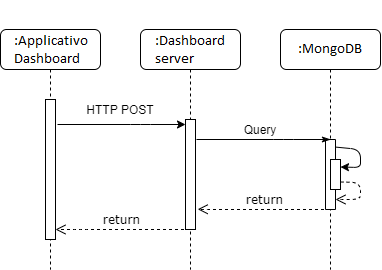
\includegraphics[width=0.65\textwidth]{img/diagramma sequenza dashboard server db.png}
  \caption{Interazione tra l'applicativo Dashboard, Dashboard server e MongoDB}
\end{figure}
\noindent Affrontiamo ora nel dettaglio struttura e funzionamento dell'applicativo Dashboard e di Dashboard server.
\vspace{10mm}
\subsection{Applicativo Dashboard}
Come struttura del progetto è stato utilizzato un approccio \emph{feature based}; tale approccio organizza i file in due categorie:
\begin{itemize}
  \item \textbf{Feature}\\
  {Una feature identifica una funzionalità offerta dal sistema.}
  \item \textbf{Componenti}\\
  {Un componente viene utilizzato da una feature per eseguire la sua funzionalità o, alternativamente, da altri componenti.}
\end{itemize}
Il progetto risulta quindi strutturato come segue:
\vspace{5mm}
\dirtree{%
.1 src.
.2 components.
.3 common.css.
.3 CommonComponent1.js.
.3 CommonComponent2.js.
.3 ....
.2 features.
.3 feature1.
.4 Feature1Component1.js.
.4 Feature1Component2.js.
.4 ....
.4 feature1Slice.js.
.4 feature1.css.
.3 feature2.
.4 ....
.3 store.
.4 index.js.
.4 reducers.js.
.3 utils.
.3 tests.
.3 index.js.
}
\vspace{5mm}
\noindent Possiamo notare che per ogni feature viene creato un file Slice.\newline 
Come anticipato precedentemente (\emph{sezione 4.2.2}), attraverso lo Slice (fornitoci da Redux Toolkit) è possibile definire comodamente reducers, azioni sincrone e azioni asincrone (Thunk).\newline
Nella cartella \emph{store} inoltre troviamo il file \emph{reducers.js}, attraverso il quale combineremo i reducers contenuti in ogni Slice al fine di creare lo Store (contenuto nel file index.js).\newline
Al fine di una maggiore chiarezza si ricorda che feature e componenti vedono realizzata la loro implementazione attraverso React.\newline
Dashboad app risulta composta da tre feature:
\begin{itemize}
  \item \bf{Login}
  \item \bf{Home}
  \item \bf{Dashboard}
\end{itemize}
Analizziamo ora nel dettaglio compiti e funzionalità di ogni feature.
\subsubsection{Login}
Corrisponde al servizio di login identificato nel primo wireframe della \emph{sezione 2.3.2} (\emph{figura 2.10}).\newline
Trattandosi di una feature semplice non è risultato necessario implementare componenti a supporto di questa feature.\newline
Al fine di ottenere una user interface gradevole per l'utente finale è stata utilizzata una libreria grafica di supporto a React chiamata \emph{Ant design} \cite{documentazione_ant_design}; questa libreria viene dunque utilizzata in gran parte delle feature e dei componenti.
\subsubsection{Home}
A login effettuato il Team manager si troverà nella home.\newline
Qui vengono individuate due aree corrispondenti ad altrettanti componenti:
\begin{itemize}
  \item \emph{TopMenu}\\
  In cima alla pagina troviamo una barra contenente dei bottoni i quali, una volta premuti, permettono all'utente di accedere alle impostazioni generali di gestione (realizzate attraverso un modale a comparsa).\newline
  Sarà dunque possibile creare, modificare ed eliminare utenti da monitorare ed inserire all'interno di Team.\newline
  Analogamente le stesse operazioni di creazione, modifica ed eliminazione saranno possibili con i Team stessi.
  \item \emph{Teams}\\
  In questa sezione invece verranno visualizzati i Team creati dai Team manager attraverso il TopMenu precedentemente discusso.\newline
  Per ogni Team verrà visualizzato il nome del Team ed una lista di tutti i componenti.\newline
  Il Team manager, interagendo con un Team, accederà alla feature Dashboard.
\end{itemize}
\subsubsection{Dashboad}
La feature Dashboard, oltre a rappresentare il punto cardine dell'applicativo, risulta essere anche la più complessa.\newline
Sulla falsa riga del wireframe precedentemente discusso (\emph{figura 2.11}) risultano individuati tre componenti principali:
\begin{itemize}
  \item \emph{Settings}\\
  Qui il Team manager potrà tornare alla Home, visualizzare il nome del team ed accedere alle impostazioni del team.\newline
  Queste ultime sono state divise a loro volta in due componenti più semplici:
  \begin{itemize}
    \item \emph{UserSettings}\\
    Qui il Team manager potrà aggiungere e rimuovere utenti dal team.\newline
    È importante sottolineare nuovamente che un Utente non potrà inviare segnali verso la piattaforma attraverso l'App di registrazione finchè un Team manager non l'avrà inserito in un team.
    \item \emph{DashboardSettings}\\
    Attraverso questo componente il Team manager sarà in grado di modificare delle impostazioni strettamente legate alla visualizzazione dei dati, ad esempio modificando l'intervallo temporale delle informazioni mostrate a schermo.
  \end{itemize}
  \item \emph{UserArea}\\
  In quest'area saranno visualizzati i dati relativi ad ogni componente del team.\newline
  Vi sono tre informazioni mostrate a schermo, ognuna a sua volta implementata come un componente:
  \begin{itemize}
    \item \emph{ConnectionStatus}\\
    Descrive lo stato della connessione dell'Utente.\newline
    Nella prima versione dell'applicativo lo stato della connessione risulta binario (online e offline), ma in versioni future verrà indicata anche la qualità del segnale inviato (corrispondente ad un posizionamento ottimo o pessimo del caschetto Muse).
    \item \emph{MeanWorkload}\\
    Attraverso un grafico a torta viene indicato il valore medio del carico cognitivo dell'Utente.\newline
    Trattandosi di un valore compreso in un intervallo chiuso da -1 a 1 il grafico si riempirà in senso orario all'aumentare di valori positivi ed in senso antiorario al diminuire di valori negativi, differenziando anche il colore in base al segno.\newline
    Inoltre, superata una certa soglia critica pericolosa per l'Utente il colore del grafico varia ulteriormente, segnalandolo all'attenzione del Team manager.
    \item \emph{SessionFatigue}\\
    L'affaticamento nella sessione di lavoro viene espresso attraverso lo stesso grafico a torta esplicato sopra ma in un range di valori differenti.
  \end{itemize}
  Interagendo con l'area di un Utente verrà cambiata modalità di visualizzazione, mostrando in un grafico cartesiano i singoli valori del carico cognitivo all'interno dell'intervallo temporale definito in DashboardSettings.\newline
  \item \emph{TeamArea}\\
  Analogamente alla UserArea, nella TeamArea verranno mostrate le stesse informazioni sopra descritte ma rappresentanti la media di tutto il team.\newline
  Vengono riutilizzati i componenti dei grafici a torta e cartesiano, aggiungendo un nuovo componente \emph{TeamStatistics} dove vengono indicate alcune statistiche del team, come ad esempio l'Utente più affaticato al momento o il numero di utenti online.
\end{itemize}
\subsection{Dashboard server}
Analizziamo ora la seconda componente del progetto, Dashboard server.\newline
L'applicativo, come discusso alla \emph{sezione 4.2}, implementa un server realizzato attraverso \emph{Node.js}.\newline
In particolare, attraverso il tool da riga di comando \emph{Node package manager} (Npm) \cite{npm}, è possibile installare il framework \emph{Express} \cite{express}.\newline
Attraverso Express ci viene fornita una funzionalità di Routing, cioè a fronte di una richiesta da parte di un client su un endpoint viene determinata la risposta del server.\newline
Il Routing è definito da un URI e da un metodo HTTP GET e/o POST. Dipendentemente dal tipo di richiesta e dall'uri richiamato si scatenerà una determinata reazione.
\subsubsection{Interfacciamento con database}
Come discusso al \emph{punto 3.3.1}, per una maggiore flessibilità si è optato per una soluzione che faccia uso di database non relazionali, in particolare utilizzando MongoDB.\newline
Attraverso l'interfaccia \emph{MongoClient} \cite{MongoClient}, fornendo le opportune configurazioni, è possibile connettersi al database MongoDB ed effettuare delle query sulle collezioni (definite al \emph{punto 3.3.1.1}).
\vspace{20mm}
\subsubsection{Endpoints}
Attraverso questi endpoints, Dashboard server riceve richieste HTTP dall'applicativo Dashboard e interroga coerentemente il database MongoDB al fine di restituire un risultato (\emph{figura 4.1}):
\vspace{8mm}
\begin{itemize}
  \item \emph{\bf login}\\
  Argomenti: username, password\newline
  In caso di successo restituisce l'identificativo dell'organizzazione di cui il Team manager fa parte.
  \item \emph{\bf teams}\\
  Argomenti: organizationId\newline
  Restituisce una lista di Team collegati all'identificativo dell'organizzazione.
  \item \emph{\bf teamSignals}\\
  Argomenti: organizationId, teamId, start, end\newline
  Per ogni Utente all'interno di un Team restituisce i dati legati al benessere cognitivo con un timestamp compreso tra start e end.
  \item \emph{\bf usersByOrganization}\\
  Argomenti: organizationId\newline
  Restituisce tutti gli Utenti facenti parte dell'organizzazione.
  \item \emph{\bf addUserToTeam}\\
  Argomenti: userId, organizationId, teamId\newline
  Modifica i dati di un Utente collegandolo ad un Team della sua organizzazione.
  \item \emph{\bf removeUserFromTeam}\\
  Argomenti: userId, organizationId, teamId\newline
  Modifica i dati di un Utente rimuovendo il suo collegamento ad un Team della sua organizzazione.
  \item \emph{\bf addTeam}\\
  Argomenti: organizationId, teamId\newline
  Crea un nuovo team all'interno di un'organizzazione.
  \item \emph{\bf deleteTeam}\\
  Argomenti: organizationId, teamId\newline
  Elimina un Team all'interno di un'organizzazione.
  \item \emph{\bf addUser}\\
  Argomenti: organizationId, userId\newline
  Crea un nuovo Utente all'interno di un'organizzazione.
  \item \emph{\bf deleteUser}\\
  Argomenti: organizationId, userId\newline
  Elimina un Utente da un'organizzazione.
\end{itemize}